% Options for packages loaded elsewhere
\PassOptionsToPackage{unicode}{hyperref}
\PassOptionsToPackage{hyphens}{url}
%
\documentclass[
]{article}
\usepackage{amsmath,amssymb}
\usepackage{lmodern}
\usepackage{iftex}
\ifPDFTeX
  \usepackage[T1]{fontenc}
  \usepackage[utf8]{inputenc}
  \usepackage{textcomp} % provide euro and other symbols
\else % if luatex or xetex
  \usepackage{unicode-math}
  \defaultfontfeatures{Scale=MatchLowercase}
  \defaultfontfeatures[\rmfamily]{Ligatures=TeX,Scale=1}
\fi
% Use upquote if available, for straight quotes in verbatim environments
\IfFileExists{upquote.sty}{\usepackage{upquote}}{}
\IfFileExists{microtype.sty}{% use microtype if available
  \usepackage[]{microtype}
  \UseMicrotypeSet[protrusion]{basicmath} % disable protrusion for tt fonts
}{}
\makeatletter
\@ifundefined{KOMAClassName}{% if non-KOMA class
  \IfFileExists{parskip.sty}{%
    \usepackage{parskip}
  }{% else
    \setlength{\parindent}{0pt}
    \setlength{\parskip}{6pt plus 2pt minus 1pt}}
}{% if KOMA class
  \KOMAoptions{parskip=half}}
\makeatother
\usepackage{xcolor}
\usepackage[margin=1in]{geometry}
\usepackage{color}
\usepackage{fancyvrb}
\newcommand{\VerbBar}{|}
\newcommand{\VERB}{\Verb[commandchars=\\\{\}]}
\DefineVerbatimEnvironment{Highlighting}{Verbatim}{commandchars=\\\{\}}
% Add ',fontsize=\small' for more characters per line
\usepackage{framed}
\definecolor{shadecolor}{RGB}{248,248,248}
\newenvironment{Shaded}{\begin{snugshade}}{\end{snugshade}}
\newcommand{\AlertTok}[1]{\textcolor[rgb]{0.94,0.16,0.16}{#1}}
\newcommand{\AnnotationTok}[1]{\textcolor[rgb]{0.56,0.35,0.01}{\textbf{\textit{#1}}}}
\newcommand{\AttributeTok}[1]{\textcolor[rgb]{0.77,0.63,0.00}{#1}}
\newcommand{\BaseNTok}[1]{\textcolor[rgb]{0.00,0.00,0.81}{#1}}
\newcommand{\BuiltInTok}[1]{#1}
\newcommand{\CharTok}[1]{\textcolor[rgb]{0.31,0.60,0.02}{#1}}
\newcommand{\CommentTok}[1]{\textcolor[rgb]{0.56,0.35,0.01}{\textit{#1}}}
\newcommand{\CommentVarTok}[1]{\textcolor[rgb]{0.56,0.35,0.01}{\textbf{\textit{#1}}}}
\newcommand{\ConstantTok}[1]{\textcolor[rgb]{0.00,0.00,0.00}{#1}}
\newcommand{\ControlFlowTok}[1]{\textcolor[rgb]{0.13,0.29,0.53}{\textbf{#1}}}
\newcommand{\DataTypeTok}[1]{\textcolor[rgb]{0.13,0.29,0.53}{#1}}
\newcommand{\DecValTok}[1]{\textcolor[rgb]{0.00,0.00,0.81}{#1}}
\newcommand{\DocumentationTok}[1]{\textcolor[rgb]{0.56,0.35,0.01}{\textbf{\textit{#1}}}}
\newcommand{\ErrorTok}[1]{\textcolor[rgb]{0.64,0.00,0.00}{\textbf{#1}}}
\newcommand{\ExtensionTok}[1]{#1}
\newcommand{\FloatTok}[1]{\textcolor[rgb]{0.00,0.00,0.81}{#1}}
\newcommand{\FunctionTok}[1]{\textcolor[rgb]{0.00,0.00,0.00}{#1}}
\newcommand{\ImportTok}[1]{#1}
\newcommand{\InformationTok}[1]{\textcolor[rgb]{0.56,0.35,0.01}{\textbf{\textit{#1}}}}
\newcommand{\KeywordTok}[1]{\textcolor[rgb]{0.13,0.29,0.53}{\textbf{#1}}}
\newcommand{\NormalTok}[1]{#1}
\newcommand{\OperatorTok}[1]{\textcolor[rgb]{0.81,0.36,0.00}{\textbf{#1}}}
\newcommand{\OtherTok}[1]{\textcolor[rgb]{0.56,0.35,0.01}{#1}}
\newcommand{\PreprocessorTok}[1]{\textcolor[rgb]{0.56,0.35,0.01}{\textit{#1}}}
\newcommand{\RegionMarkerTok}[1]{#1}
\newcommand{\SpecialCharTok}[1]{\textcolor[rgb]{0.00,0.00,0.00}{#1}}
\newcommand{\SpecialStringTok}[1]{\textcolor[rgb]{0.31,0.60,0.02}{#1}}
\newcommand{\StringTok}[1]{\textcolor[rgb]{0.31,0.60,0.02}{#1}}
\newcommand{\VariableTok}[1]{\textcolor[rgb]{0.00,0.00,0.00}{#1}}
\newcommand{\VerbatimStringTok}[1]{\textcolor[rgb]{0.31,0.60,0.02}{#1}}
\newcommand{\WarningTok}[1]{\textcolor[rgb]{0.56,0.35,0.01}{\textbf{\textit{#1}}}}
\usepackage{graphicx}
\makeatletter
\def\maxwidth{\ifdim\Gin@nat@width>\linewidth\linewidth\else\Gin@nat@width\fi}
\def\maxheight{\ifdim\Gin@nat@height>\textheight\textheight\else\Gin@nat@height\fi}
\makeatother
% Scale images if necessary, so that they will not overflow the page
% margins by default, and it is still possible to overwrite the defaults
% using explicit options in \includegraphics[width, height, ...]{}
\setkeys{Gin}{width=\maxwidth,height=\maxheight,keepaspectratio}
% Set default figure placement to htbp
\makeatletter
\def\fps@figure{htbp}
\makeatother
\setlength{\emergencystretch}{3em} % prevent overfull lines
\providecommand{\tightlist}{%
  \setlength{\itemsep}{0pt}\setlength{\parskip}{0pt}}
\setcounter{secnumdepth}{-\maxdimen} % remove section numbering
\ifLuaTeX
  \usepackage{selnolig}  % disable illegal ligatures
\fi
\IfFileExists{bookmark.sty}{\usepackage{bookmark}}{\usepackage{hyperref}}
\IfFileExists{xurl.sty}{\usepackage{xurl}}{} % add URL line breaks if available
\urlstyle{same} % disable monospaced font for URLs
\hypersetup{
  pdftitle={Prova P2 - MAF 172 - 2022-2},
  pdfauthor={Erich Müller Dutra - Matrícula 4908},
  hidelinks,
  pdfcreator={LaTeX via pandoc}}

\title{Prova P2 - MAF 172 - 2022-2}
\author{Erich Müller Dutra - Matrícula 4908}
\date{2022-11-07}

\begin{document}
\maketitle

{
\setcounter{tocdepth}{2}
\tableofcontents
}
\hypertarget{introduuxe7uxe3o}{%
\section{- Introdução}\label{introduuxe7uxe3o}}

Nesta seção, estudamos a relação entre diferentes variáveis aplicadas à
ciência de dados no R. Neste trabalho, investiguei a relação entre notas
de corte para acesso ao curso de administração através do SiSU,
investimentos educacionais, população e IDH. Foram coletadas 8 amostras
através de dados públicos disponíveis na plataforma do SiSU, portal da
transparência e IBGE.

\hypertarget{objetivo}{%
\section{- Objetivo}\label{objetivo}}

A principal motivação é estudar se há relação direta entre dados das
localidades e a concorrência para o curso de administração através do
SiSU.

\hypertarget{descriuxe7uxe3o-das-variuxe1veis}{%
\section{- Descrição das
Variáveis}\label{descriuxe7uxe3o-das-variuxe1veis}}

\hypertarget{fonte}{%
\subsection{- Fonte}\label{fonte}}

Os dados coletados foram obtidos através das seguintes fontes: *
\url{https://sisu.mec.gov.br/\#/relatorio\#onepage} *
\url{https://cidades.ibge.gov.br} *
\url{https://www.portaltransparencia.gov.br/funcoes/12-educacao?ano=2020}

\hypertarget{preparauxe7uxe3o-do-ambiente}{%
\subsection{- Preparação do
ambiente}\label{preparauxe7uxe3o-do-ambiente}}

A partir daqui, iremos analisar a relação entre as variáveis.
Inicialmente, vamos preparar o ambiente.

\begin{Shaded}
\begin{Highlighting}[]
\CommentTok{\# Define o diretório de trabalho}
\CommentTok{\#setwd("\textasciitilde{}Documents/Erich/GitHub/MAF\_172") }

\CommentTok{\# Instalando dependências}
\FunctionTok{library}\NormalTok{(pacman)}
\FunctionTok{p\_load}\NormalTok{(}\AttributeTok{char=}\FunctionTok{c}\NormalTok{(}\StringTok{"DescTools"}\NormalTok{,}\StringTok{"readxl"}\NormalTok{,}\StringTok{"janitor"}\NormalTok{, }\StringTok{"psych"}\NormalTok{, }\StringTok{"corrr"}\NormalTok{, }\StringTok{"ggplot2"}\NormalTok{, }\StringTok{"dplyr"}\NormalTok{, }\StringTok{"caret"}\NormalTok{, }\StringTok{"corrplot"}\NormalTok{,}\StringTok{"spatstat"}\NormalTok{, }\StringTok{"maptools"}\NormalTok{, }\StringTok{"gstat"}\NormalTok{, }\StringTok{"foreign"}\NormalTok{, }\StringTok{"geoR"}\NormalTok{,}\StringTok{"moments"}\NormalTok{,}\StringTok{"scatterplot3d"}\NormalTok{,}\StringTok{"tcltk2"}\NormalTok{, }\StringTok{"sp"}\NormalTok{, }\StringTok{"rgdal"}\NormalTok{, }\StringTok{"raster"}\NormalTok{, }\StringTok{"doParallel"}\NormalTok{, }\StringTok{"GGally"}\NormalTok{))}
\end{Highlighting}
\end{Shaded}

\hypertarget{leitura-dos-dados}{%
\subsection{- Leitura dos dados}\label{leitura-dos-dados}}

Faremos então a leitura dos dados que estão armazenados em um arquivo de
texto (.txt).

\begin{Shaded}
\begin{Highlighting}[]
\CommentTok{\# Importando os dados}
\NormalTok{dados }\OtherTok{=} \FunctionTok{read.table}\NormalTok{(}\StringTok{"../dados\_prova.txt"}\NormalTok{, }\AttributeTok{head=}\NormalTok{T)}
\FunctionTok{str}\NormalTok{(dados)}
\end{Highlighting}
\end{Shaded}

\begin{verbatim}
## 'data.frame':    8 obs. of  5 variables:
##  $ NOTACORTE    : num  754 706 733 727 688 ...
##  $ INVESTIMENTO : int  1360782 65865 90000 293600 459714 337270 248592 835479
##  $ NUMHABITANTES: int  6775561 12330000 2722000 1492530 278264 261501 343132 402912
##  $ IDH          : num  0.799 0.805 0.81 0.805 0.694 0.764 0.739 0.72
##  $ CIDADE       : chr  "Rio de Janeiro" "São Paulo" "Belo Horizonte" "Porto Alegre" ...
\end{verbatim}

\begin{Shaded}
\begin{Highlighting}[]
\CommentTok{\# Leitura dos dados importados}
\NormalTok{dados.rls }\OtherTok{=}\NormalTok{ dados[}\DecValTok{1}\SpecialCharTok{:}\DecValTok{4}\NormalTok{]}
\FunctionTok{names}\NormalTok{(dados.rls)}
\end{Highlighting}
\end{Shaded}

\begin{verbatim}
## [1] "NOTACORTE"     "INVESTIMENTO"  "NUMHABITANTES" "IDH"
\end{verbatim}

\hypertarget{processamento-dos-dados}{%
\subsection{- Processamento dos dados}\label{processamento-dos-dados}}

Vamos agora processar os dados obtidos de três formas, sendo duas delas
através de correlação de matriz linear e a outra como correlação não
linear.

\hypertarget{matriz-de-correlauxe7uxe3o-linear}{%
\subsubsection{- Matriz de correlação
linear}\label{matriz-de-correlauxe7uxe3o-linear}}

\begin{Shaded}
\begin{Highlighting}[]
\CommentTok{\# Processamento em paralelo}
\NormalTok{cl }\OtherTok{\textless{}{-}} \FunctionTok{makePSOCKcluster}\NormalTok{(}\DecValTok{4}\NormalTok{)}
\FunctionTok{registerDoParallel}\NormalTok{(cl)}
\CommentTok{\# Aqui começa o procedimento}
\NormalTok{df2 }\OtherTok{\textless{}{-}} \FunctionTok{cor}\NormalTok{(dados.rls, }\AttributeTok{use =} \StringTok{"na.or.complete"}\NormalTok{)}
\FunctionTok{corrplot}\NormalTok{(df2, }\AttributeTok{order=}\StringTok{"alphabet"}\NormalTok{, }\AttributeTok{method=}\StringTok{"circle"}\NormalTok{, }\AttributeTok{tl.pos=}\StringTok{"td"}\NormalTok{, }\AttributeTok{type=}\StringTok{"upper"}\NormalTok{, }
         \AttributeTok{tl.col=}\StringTok{"black"}\NormalTok{, }\AttributeTok{tl.cex=}\FloatTok{0.9}\NormalTok{, }\AttributeTok{tl.srt=}\DecValTok{45}\NormalTok{, }
         \AttributeTok{addCoef.col=}\StringTok{"orange"}\NormalTok{, }\AttributeTok{addCoefasPercent =} \ConstantTok{TRUE}\NormalTok{, }\AttributeTok{diag =} \ConstantTok{TRUE}\NormalTok{,}
         \AttributeTok{sig.level=}\FloatTok{0.995}\NormalTok{, }\AttributeTok{p.mat =} \DecValTok{1}\SpecialCharTok{{-}}\FunctionTok{abs}\NormalTok{(df2),}\AttributeTok{insig =} \StringTok{"blank"}\NormalTok{)}
\end{Highlighting}
\end{Shaded}

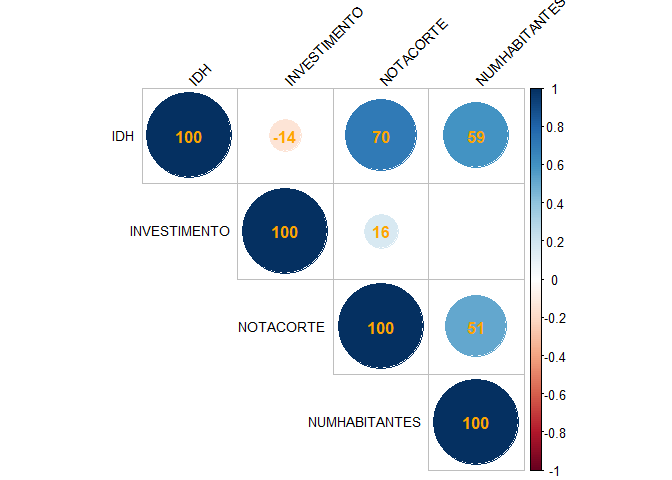
\includegraphics{Script-Rmd-Aula-7_files/figure-latex/unnamed-chunk-3-1.pdf}

\begin{Shaded}
\begin{Highlighting}[]
\CommentTok{\# Aqui termina o procedimento}
\FunctionTok{stopCluster}\NormalTok{(cl)}
\end{Highlighting}
\end{Shaded}

Nessa análise, pudemos observar que a maior relação linear encontrada se
dá entre a nota de corte e o IDH.

\hypertarget{outra-matriz-de-correlauxe7uxe3o-linear}{%
\subsubsection{- Outra Matriz de correlação
linear}\label{outra-matriz-de-correlauxe7uxe3o-linear}}

\begin{Shaded}
\begin{Highlighting}[]
\CommentTok{\# Outra Matriz de Correlacao}

\NormalTok{cl }\OtherTok{\textless{}{-}} \FunctionTok{makePSOCKcluster}\NormalTok{(}\DecValTok{4}\NormalTok{); }\FunctionTok{registerDoParallel}\NormalTok{(cl)}
\CommentTok{\# Aqui começa o procedimento}
\FunctionTok{ggpairs}\NormalTok{(dados.rls)}
\end{Highlighting}
\end{Shaded}

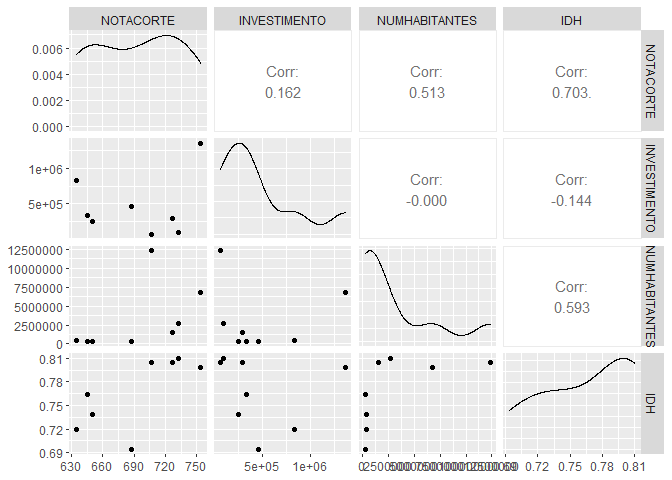
\includegraphics{Script-Rmd-Aula-7_files/figure-latex/unnamed-chunk-4-1.pdf}

\begin{Shaded}
\begin{Highlighting}[]
\CommentTok{\# Aqui termina o procedimento}
\FunctionTok{stopCluster}\NormalTok{(cl)}
\end{Highlighting}
\end{Shaded}

Através dessa matriz, podemos ver como os dados se relacionam e o grau
de correlação.

\hypertarget{matriz-de-correlauxe7uxe3o-nuxe3o-linear}{%
\subsubsection{- Matriz de correlação não
linear}\label{matriz-de-correlauxe7uxe3o-nuxe3o-linear}}

\begin{Shaded}
\begin{Highlighting}[]
\FunctionTok{par}\NormalTok{(}\AttributeTok{mfrow=}\FunctionTok{c}\NormalTok{(}\DecValTok{1}\NormalTok{,}\DecValTok{1}\NormalTok{))}
\FunctionTok{par}\NormalTok{(}\AttributeTok{mar=}\FunctionTok{c}\NormalTok{(}\DecValTok{8}\NormalTok{,}\DecValTok{4}\NormalTok{,}\DecValTok{6}\NormalTok{,}\DecValTok{4}\NormalTok{))}
\CommentTok{\# Processamento em paralelo}
\NormalTok{cl }\OtherTok{\textless{}{-}} \FunctionTok{makePSOCKcluster}\NormalTok{(}\DecValTok{4}\NormalTok{)}
\FunctionTok{registerDoParallel}\NormalTok{(cl)}
\CommentTok{\# Aqui começa o procedimento}
\CommentTok{\# Função de Lopez{-}Paz (2013)}
\NormalTok{rdc }\OtherTok{\textless{}{-}} \ControlFlowTok{function}\NormalTok{(x,y,}\AttributeTok{k=}\DecValTok{20}\NormalTok{,}\AttributeTok{s=}\DecValTok{1}\SpecialCharTok{/}\DecValTok{6}\NormalTok{,}\AttributeTok{f=}\NormalTok{sin) \{}
  \FunctionTok{set.seed}\NormalTok{(}\DecValTok{313}\NormalTok{)}
\NormalTok{  x }\OtherTok{\textless{}{-}} \FunctionTok{cbind}\NormalTok{(}\FunctionTok{apply}\NormalTok{(}\FunctionTok{as.matrix}\NormalTok{(x),}\DecValTok{2}\NormalTok{,}\ControlFlowTok{function}\NormalTok{(u)}\FunctionTok{rank}\NormalTok{(u)}\SpecialCharTok{/}\FunctionTok{length}\NormalTok{(u)),}\DecValTok{1}\NormalTok{)}
\NormalTok{  y }\OtherTok{\textless{}{-}} \FunctionTok{cbind}\NormalTok{(}\FunctionTok{apply}\NormalTok{(}\FunctionTok{as.matrix}\NormalTok{(y),}\DecValTok{2}\NormalTok{,}\ControlFlowTok{function}\NormalTok{(u)}\FunctionTok{rank}\NormalTok{(u)}\SpecialCharTok{/}\FunctionTok{length}\NormalTok{(u)),}\DecValTok{1}\NormalTok{)}
\NormalTok{  x }\OtherTok{\textless{}{-}}\NormalTok{ s}\SpecialCharTok{/}\FunctionTok{ncol}\NormalTok{(x)}\SpecialCharTok{*}\NormalTok{x}\SpecialCharTok{\%*\%}\FunctionTok{matrix}\NormalTok{(}\FunctionTok{rnorm}\NormalTok{(}\FunctionTok{ncol}\NormalTok{(x)}\SpecialCharTok{*}\NormalTok{k),}\FunctionTok{ncol}\NormalTok{(x))}
\NormalTok{  y }\OtherTok{\textless{}{-}}\NormalTok{ s}\SpecialCharTok{/}\FunctionTok{ncol}\NormalTok{(y)}\SpecialCharTok{*}\NormalTok{y}\SpecialCharTok{\%*\%}\FunctionTok{matrix}\NormalTok{(}\FunctionTok{rnorm}\NormalTok{(}\FunctionTok{ncol}\NormalTok{(y)}\SpecialCharTok{*}\NormalTok{k),}\FunctionTok{ncol}\NormalTok{(y))}
  \FunctionTok{cancor}\NormalTok{(}\FunctionTok{cbind}\NormalTok{(}\FunctionTok{f}\NormalTok{(x),}\DecValTok{1}\NormalTok{),}\FunctionTok{cbind}\NormalTok{(}\FunctionTok{f}\NormalTok{(y),}\DecValTok{1}\NormalTok{))}\SpecialCharTok{$}\NormalTok{cor[}\DecValTok{1}\NormalTok{]}
\NormalTok{\}}
\CommentTok{\# Tabela é o data.frame}
\NormalTok{tabela }\OtherTok{=}\NormalTok{ dados.rls}
\NormalTok{correl\_nao\_linear }\OtherTok{\textless{}{-}} \ControlFlowTok{function}\NormalTok{ (tabela) \{}
\NormalTok{  c }\OtherTok{=} \FunctionTok{c}\NormalTok{(}\StringTok{"peraser"}\NormalTok{)}
\NormalTok{  mcnl }\OtherTok{=} \FunctionTok{matrix}\NormalTok{(}\AttributeTok{nrow =} \FunctionTok{ncol}\NormalTok{(tabela), }\AttributeTok{ncol =} \FunctionTok{ncol}\NormalTok{(tabela))  }
  \ControlFlowTok{for}\NormalTok{ (i }\ControlFlowTok{in} \DecValTok{1}\SpecialCharTok{:}\FunctionTok{ncol}\NormalTok{(tabela)) \{}
    \ControlFlowTok{for}\NormalTok{ (j }\ControlFlowTok{in} \DecValTok{1}\SpecialCharTok{:}\FunctionTok{ncol}\NormalTok{(tabela)) \{}
\NormalTok{      mcnl[i,j] }\OtherTok{=} \FunctionTok{rdc}\NormalTok{(tabela[,i],tabela[,j])}
\NormalTok{    \}}
\NormalTok{  \}}
\NormalTok{  mcnl }\OtherTok{=}\FunctionTok{as.data.frame}\NormalTok{(mcnl)}
  \FunctionTok{colnames}\NormalTok{(mcnl) }\OtherTok{=} \FunctionTok{colnames}\NormalTok{(tabela)}
  \FunctionTok{rownames}\NormalTok{(mcnl) }\OtherTok{=} \FunctionTok{colnames}\NormalTok{(tabela)}
  \FunctionTok{return}\NormalTok{(mcnl)}
\NormalTok{\}}
\FunctionTok{par}\NormalTok{(}\AttributeTok{mfrow=}\FunctionTok{c}\NormalTok{(}\DecValTok{1}\NormalTok{,}\DecValTok{1}\NormalTok{))}
\NormalTok{cornl }\OtherTok{=} \FunctionTok{correl\_nao\_linear}\NormalTok{(tabela)}
\FunctionTok{corrplot}\NormalTok{(}\FunctionTok{as.matrix}\NormalTok{(cornl),}\AttributeTok{is.corr =}\NormalTok{ F, }\AttributeTok{method=}\StringTok{"circle"}\NormalTok{, }\AttributeTok{tl.srt=}\DecValTok{45}\NormalTok{,}
         \AttributeTok{tl.pos=}\StringTok{"lt"}\NormalTok{, }\AttributeTok{type=}\StringTok{"upper"}\NormalTok{,}\AttributeTok{tl.col=}\StringTok{"black"}\NormalTok{, }\AttributeTok{addCoefasPercent =} \ConstantTok{TRUE}\NormalTok{,}
         \AttributeTok{sig.level=}\FloatTok{0.995}\NormalTok{, }\AttributeTok{addCoef.col=}\StringTok{"orange"}\NormalTok{)}
\end{Highlighting}
\end{Shaded}

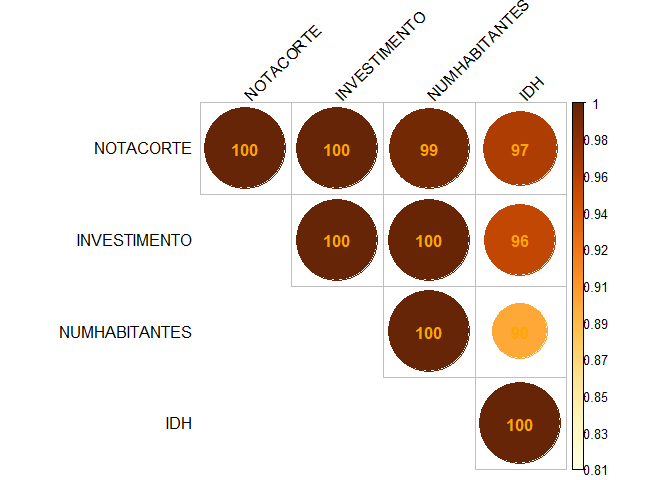
\includegraphics{Script-Rmd-Aula-7_files/figure-latex/unnamed-chunk-5-1.pdf}

\begin{Shaded}
\begin{Highlighting}[]
\CommentTok{\# Aqui termina o procedimento}
\FunctionTok{stopCluster}\NormalTok{(cl)}
\end{Highlighting}
\end{Shaded}

Através dessa análise podemos concluir que as variáveis observadas
possuem alto grau de correlação não linear, sendo as maiores delas a
nota de corte com relação ao investimento e o investimento com relação
ao número de habitantes.

\hypertarget{regressuxe3o-linear-simples}{%
\section{- Regressão Linear Simples}\label{regressuxe3o-linear-simples}}

Nesta seção, faremos uma simples regressão linear entre as variáveis IDH
e NOTADECORTE. Foram escolhidas essas variáveis pois são as que possuem
maior índice de correlação linear.

O código abaixo realiza o diagrama de dispersão dos referidos dados.

\begin{Shaded}
\begin{Highlighting}[]
\NormalTok{resp }\OtherTok{=}\NormalTok{ dados.rls}\SpecialCharTok{$}\NormalTok{NOTACORTE}
\NormalTok{explic }\OtherTok{=}\NormalTok{ dados.rls}\SpecialCharTok{$}\NormalTok{IDH}
\CommentTok{\# Gerando o gráfico}
\FunctionTok{par}\NormalTok{(}\AttributeTok{mfrow=}\FunctionTok{c}\NormalTok{(}\DecValTok{1}\NormalTok{,}\DecValTok{1}\NormalTok{))}
\FunctionTok{plot}\NormalTok{(explic, resp, }\AttributeTok{main=}\StringTok{"Diagrama de Dispersão"}\NormalTok{, }
     \AttributeTok{xlab =} \StringTok{"IDH"}\NormalTok{, }\AttributeTok{ylab =} \StringTok{"NOTA DE CORTE"}\NormalTok{) }
\end{Highlighting}
\end{Shaded}

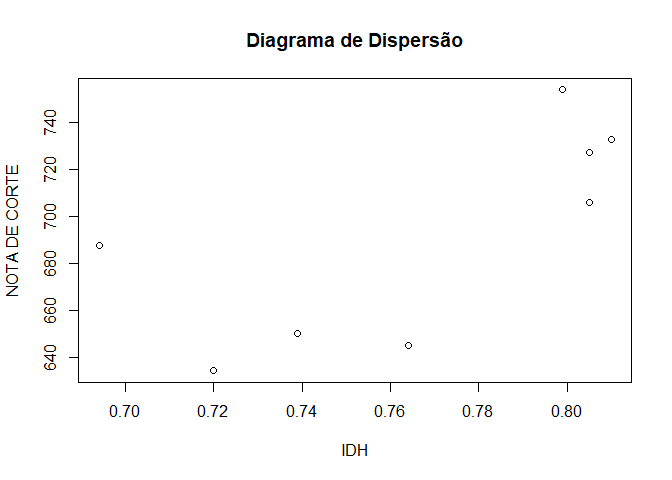
\includegraphics{Script-Rmd-Aula-7_files/figure-latex/unnamed-chunk-6-1.pdf}

Com o código abaixo, faremos uma estimativa da função linear que melhor
se adequa aos dados.

\begin{Shaded}
\begin{Highlighting}[]
\NormalTok{(}\AttributeTok{rls =} \FunctionTok{lm}\NormalTok{(resp}\SpecialCharTok{\textasciitilde{}}\NormalTok{explic))}
\end{Highlighting}
\end{Shaded}

\begin{verbatim}
## 
## Call:
## lm(formula = resp ~ explic)
## 
## Coefficients:
## (Intercept)       explic  
##       151.9        704.4
\end{verbatim}

Obtivemos portanto uma função do tipo \(f(x) = 704.4x + 151.9\). Sendo
\(151.9\) a intersecção da reta com o eixo das ordenadas e \(704.4\) a
taxa de variação, ou seja, a cada aumento de \(0.1\) no IDH, a nota de
corte cresce, em média, \(70.44\).

O código abaixo mostrará a reta definida pela função acima plotada no
gráfico de dispersão.

\begin{Shaded}
\begin{Highlighting}[]
\FunctionTok{par}\NormalTok{(}\AttributeTok{mar=}\FunctionTok{c}\NormalTok{(}\DecValTok{6}\NormalTok{,}\DecValTok{4}\NormalTok{,}\DecValTok{4}\NormalTok{,}\DecValTok{4}\NormalTok{))}
\FunctionTok{plot}\NormalTok{(explic, resp)}
\FunctionTok{abline}\NormalTok{(rls)}
\FunctionTok{text}\NormalTok{(}\DecValTok{3}\NormalTok{,}\DecValTok{90}\NormalTok{,}\FunctionTok{expression}\NormalTok{(}\StringTok{"f(x) = 704.4x + 151.9"}\NormalTok{))}
\end{Highlighting}
\end{Shaded}

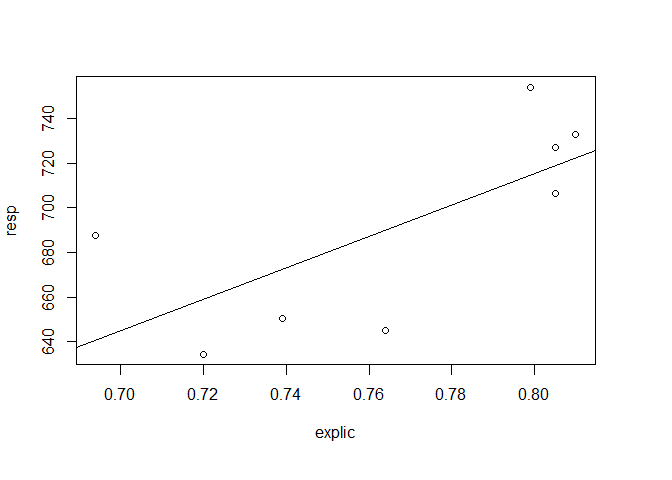
\includegraphics{Script-Rmd-Aula-7_files/figure-latex/unnamed-chunk-8-1.pdf}

A reta não intercepta perfeitamente os pontos, entretanto é uma
aproximação razoável para descrever as notas de corte em função do IDH.

\end{document}
